%
% T�TULO DEL CAP�TULO
%
\chapter{Performance \& Experimental Results
	\label{chapter_4}
}

In this chapter we will delve in the obtained performance results in the two test machines, as well as taking a look at the experimental results obtained for a couple of test datasets. The images that will be used for testing are described in \autoref{dataset_table}. %TODO Obtained from middlebury datasets.

\begin{table}[h]
\centering
\begin{tabular}{clcc}
\toprule
& Dataset & Width & Height \\
\midrule
 \parbox{2.5cm}{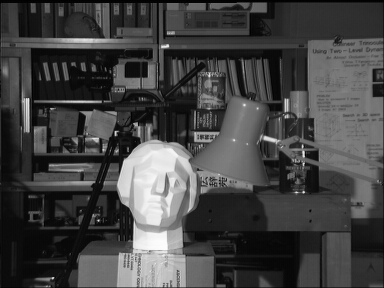
\includegraphics[width=\linewidth]{../data/tsukuba_l.png}} & Tsukuba & 384  & 288 \\[1cm]
 \parbox{2.5cm}{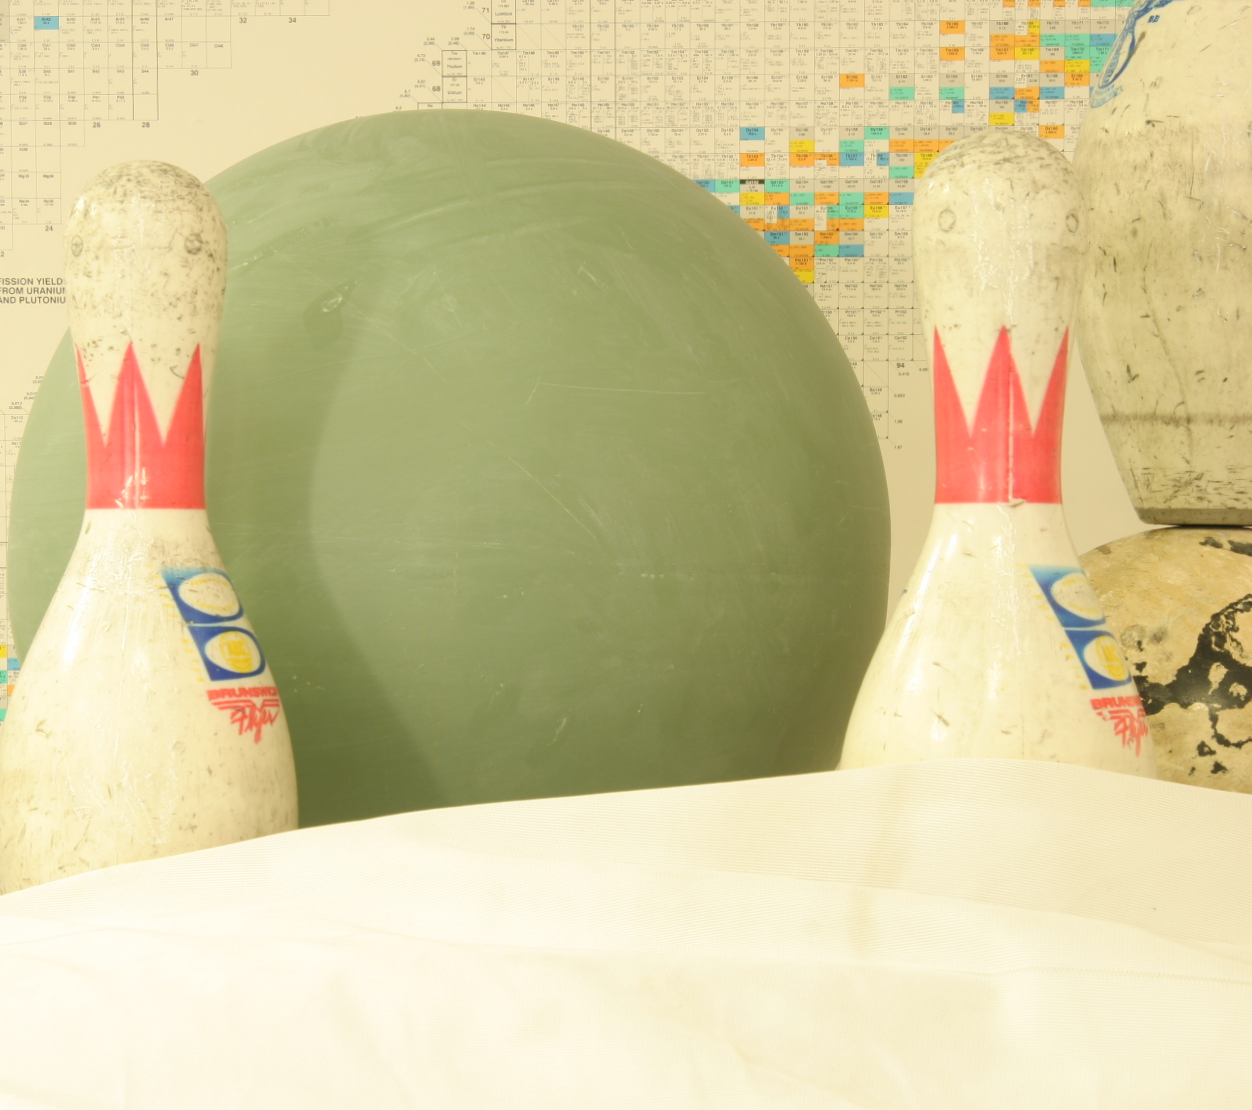
\includegraphics[width=\linewidth]{../data/bowling_l.png}} & Bowling & 1252  & 1110 \\[1cm]
\bottomrule
\end{tabular}
\caption{Datasets used in our tests.}
\label{dataset_table}
\end{table}

\section{Performance Results}

Two computers with different hardware were used for testing. The first, \textbf{Computer 1} has the following specs:

\begin{itemize}
	\item Intel Core i7-3770 CPU (4 cores, 8 threads)
	\item NVIDIA GT 640 graphics card
	\item 16 GB of 1600 MHz DDR3 RAM
	\item WDC WD10EZRX HDD
\end{itemize} 

The second, \textbf{Computer 2} has the following specifications:

\begin{itemize}
	\item Intel Core i7-4930K CPU (6 cores, 12 threads)
	\item NVIDIA GTX 780Ti graphics card
	\item 16 GB of 2133 MHz DDR3 RAM
	\item WD Caviar Black HDD
\end{itemize} 

The operating system used to run the tests was Windows 7 x64, with the VC{}\verb!++! v110 compiler.

\section{Experimental Results}

